\chapter{Desenvolvemento}
\label{cap:desarrollo}

% TFG BREVE: Es conveniente comenzar el capítulo un un par de párrafos que explique su contenido. Por ejemplo: "En este capítulo se presenta en desarrollo del proyecto realizado. Comenzaremos explicando las tecnologías utilizadas para, posteriormente, detallar ...."
Neste capítulo preséntase o desenvolvemento do proxecto realizado. Comenzaremos cas eleccións tecnolóxicas que se tomaron para acadar o mellor resultado que cumpra os requirimentos recollidos. Despois detallaremos o proceso de desenvolvemento explicando a resolución das problemáticas atopadas e a implementación dos diferentes prototipos ata chegar ao resultado conseguido.  

\section{Tecnologías}
% En el TFG se suele poner un capítulo completo dedicado a las tecnologías empleadas, pero en el TFG BREVE se hará en esta sección. Se pretende resumir las tecnologías y explicar por qué se han elegido. Hay que evitar hacer copy-paste de web. Además, es importante poner referencias bibliográficas utilizando este formato: \cite{ErlangBook,ErlangWebBook}. 
Para a implementación do sistema hardware que fai de teclado de piano o microcontrolador empregado foi o ESP32 como o da figura \ref{fig:esp32}. Este microcontrolador é un SoC e é moi valorado tanto no entorno educativo coma no empresarial pola súa relación prezo-prestacións. Mantendo un prezo por debaixo dos 10 euros ofrece un sistema de baixo consumo, con unha cantidade notable de pins para o seu reducido tamaño, soporte para as contornas de desenvolvemento de Arduino e con outras contornas como Thonny, a utilizada nas sesións de prácticas da materia; e como factor máis destacable, Wifi e Bluetooth integrados sen necesidade de un módulo a maiores\cite{ESP32MX}. Ademais destas características a elección foi motivada tamén porque é a placa utilizada en algunhas sesións de prácticas da materia.
Para a súa programación empregaremos empregaremos Micropython, unha implementación de Python 3 orientada a microcontroladores \cite{MicroPython}. Neste caso tamén usamos esta contorna na materia. Ademais, permítenos programar de forma moi flexible e cómoda cunha linguaxe de moi alto nivel co que xa estou familiarizado. Como o programa a implementar é sinxelo e non empregamos unha gran cantidade de recursos podémonos permitir utilizar este entorno menos eficiente pero máis cómodo co que traballar.

\begin{figure}[hp!]
  \centering
  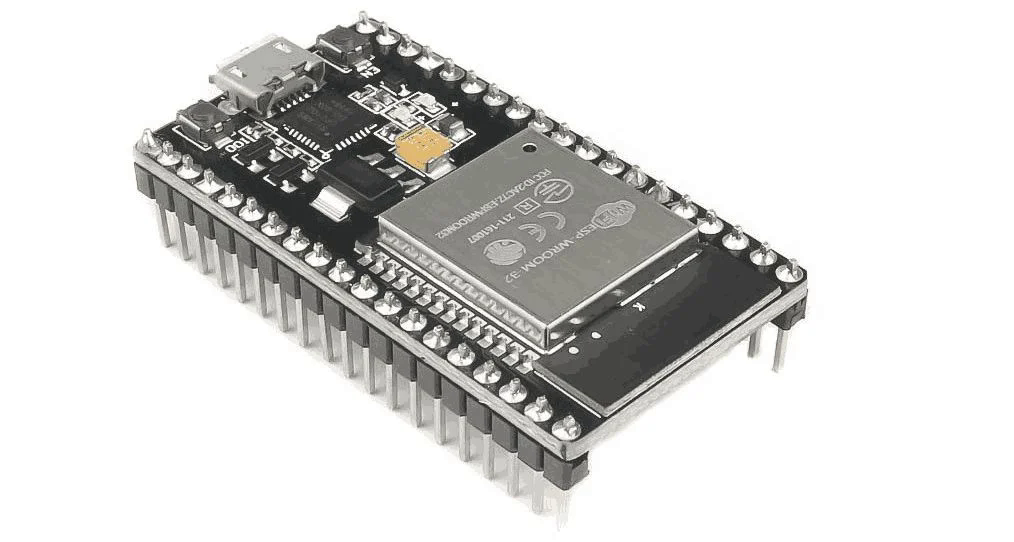
\includegraphics[width=0.75\textwidth]{imaxes/ESP32.png}
  \caption{Imaxe dun ESP32}
  \label{fig:esp32}
\end{figure}

\newline{}\newline{}
Para o desenvolvemento da aplicación principal a necesidade de cumprir cuns estándares de accesibilidade importantes fixeron que a elección da plataforma para desenvolver a vista fose unha tecnoloxía web. A web é das contornas con máis ferramentas para as persoas con necesidades de accesibilidade específicas. Iniciativas e estándares como Web Accessibility Initiative \cite{WAI} do W3C fan que as utilidades para estas persoas sexan numerosas e o traballo dos programadores mínimo. Frente á web, outras plataformas non teñen tan desenvoltos estes aspectos.

Para poder interactuar co sistema operativo para o control do sistema hardware requirimos que esta vista web se execute fóra da contorna illada dun navegador. Existen varias tecnoloxías que nos permiten facer isto. A máis importante sen dúbida é Electron \cite{Electron}. Esta tecnoloxía empaqueta o navegador Chromium e a contorna de execución de Javascript Nodejs para obter unha plataforma para aplicacións multiplataforma sen código específico de cada plataforma e permitindo compartir unha vista entre a versión web e a versión de escritorio ou móbil. Úsase por exemplo, en VSCode, en Discord ou en Microsoft Teams. 

A plataforma finalmente elixida é unha alternativa a esta última ferramenta, pero que soluciona un dos maiores problemas desta. Esta alternativa é Tauri \cite{Tauri}.
Tauri permite crear aplicacións multiplataforma sen necesidade de ter empaquetados moi pesados. Mentres cada aplicación que utiliza Electron empaqueta o seu propio Chromium e Nodejs, Tauri utiliza a vista web nativa do sistema operativo e o seu núcleo é un binario codificado en Rust \cite{Rust} moi livián, comunicados mediante o paso de mensaxes entre diferentes procesos, como se mostra na figura \ref{fig:TauriIPC}. Isto permite pasar de tamaños de aplicacións da orde de centos de megabytes a soamente uns poucos megabytes. Isto tamén produce inconvenientes, xa que ao depender da vista web nativa, esta non será totalmente igual en todos os sistema, debido ás diferentes implementacións e versións dos motores de renderizado que utiliza cada sistema operativo. Por exemplo, en Windows utilízase o motor WebView2 (baseado en Edge que á súa vez basease en Chromium), mentres que en macOS emprega WebKit, e en Linux úsase WebKitGTK. A pesar deste problema, elixín esta opción ao ser este un problema menor que tamén pasa na web entre diferentes navegadores e ao ser o beneficio maior ás desventaxas. 

\begin{figure}[hp!]
  \centering
  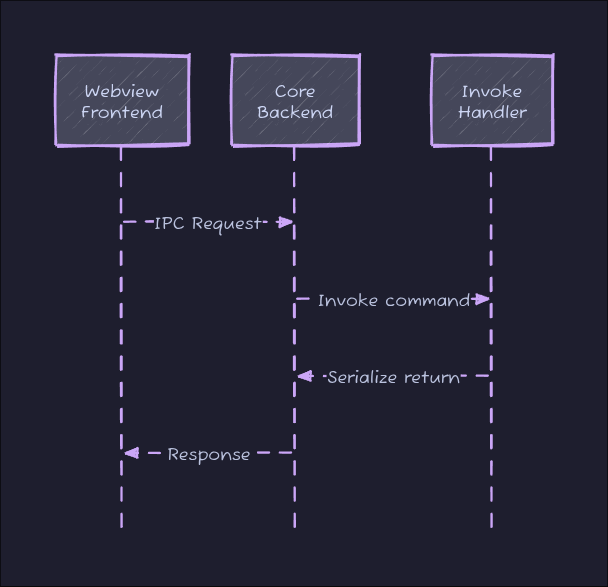
\includegraphics[width=0.75\textwidth]{imaxes/TauriIPC.png}
  \caption{Diagrama da comunicación entre procesos de Tauri}
  \label{fig:TauriIPC}
\end{figure}

Para codificar a vista usei a popular librería de UI desenvolta por Meta, React \cite{React}. Esta opción moi usada tanto a nivel nacional como internacional permítenos desenvolver aplicacións reactivas de xeito sinxelo e moi cómodo para o programador.

Para a manipulación do son utilízase a librería de manipulación de son Rodio \cite{Rodio}, que nos permite reproducir son de forma multiplataforma.

Para o control do porto serie para a comunicación co sistema hardware utilízase a librería serialport-rs \cite{Serialport}, que nos permite traballar co porto serie abstraendo as peculiaridades de cada sistema operativo. 


\section{Desarrollo}
% En el TFG suele haber varios capítulos para explicar el desarrollo realizados. Aquí lo haremos en un solo capítulo.

% En el caso de proyectos con microcontroladores, se debe indicar claramente el montaje. 

% En caso de incluir figuras, deben referenciarse de esta forma "la figura~\ref{fig:exemplo} ". Todas las figuras deben estar referenciadas en el texto.
% Se recomienda poner todas las figuras en el directorio \texttt{imaxes}.

\begin{figure}[hp!]
  \centering
  
\includegraphics[width=0.75\textwidth]{imaxes/udc.png}
  \caption{Título de la figura}
  \label{fig:exemplo}
\end{figure}

\begin{figure}[hp!]
  \centering
  \begin{subfigure}[c]{0.3\textwidth}
    
\includegraphics[angle=45,width=\textwidth]{imaxes/udc.png}
    \caption{Título figura 1}
    \label{fig:subfigura-rotada}
  \end{subfigure}
  \hspace{0.1\textwidth}
  \begin{subfigure}[c]{0.3\textwidth}
    
\includegraphics[width=\textwidth,height=3cm]{imaxes/udc.png}
    \caption{Título figura 2}
    \label{fig:subfigura-deformada}
  \end{subfigure}
  \caption{Título general de la figura}
  \label{fig:exemplo-subfiguras}
\end{figure}

% Se puede añadir partes del código que sean importantes para entender el desarrollo.

% Se pueden incluir cuadros (tablas). Los cuadros tienen que estar referenciados en el texto (por ejemplo, el cuadro \ref{tab:exemplo}).

\begin{table}[hp!]
  \centering
  \rowcolors{2}{white}{udcgray!25}
  \begin{tabular}{c|c}
  \rowcolor{udcpink!25}
  \textbf{Título de columna} & \textbf{Outro título de columna} \\\hline
  \textit{Título de fila} & Contido de celda \\
  \textit{Título de fila} & Contido de celda \\
  \textit{Título de fila} & Contido de celda \\
  \textit{Título de fila} & Contido de celda \\
  \textit{Título de fila} & Contido de celda \\
  \textit{Título de fila} & Contido de celda \\
  \end{tabular}
  \caption{Título del cuadro}
  \label{tab:exemplo}
\end{table}



